%%%%%%%%%%%%%%%%%%%%%%%%%%%%%%%%%%%%%%%%%%%%%%%%%%%%%%%%%%%%%%%%%%%%%%%%%%%%%%%%
%2345678901234567890123456789012345678901234567890123456789012345678901234567890
%        1         2         3         4         5         6         7         8

\documentclass[letterpaper, 11pt, conference, margin=1in]{ieeeconf}   % Comment this line out
                                                          % if you need a4paper
%\documentclass[a4paper, 10pt, conference]{ieeeconf}      % Use this line for a4
                                                          % paper

\IEEEoverridecommandlockouts                              % This command is only
                                                          % needed if you want to
                                                          % use the \thanks command
\overrideIEEEmargins
% See the \addtolength command later in the file to balance the column lengths
% on the last page of the document

% The following packages can be found on http:\\www.ctan.org
\usepackage{graphics} % for pdf, bitmapped graphics files
%\usepackage{epsfig} % for postscript graphics files
%\usepackage{mathptmx} % assumes new font selection scheme installed
\usepackage{times} % assumes new font selection scheme installed
%\usepackage{amsmath} % assumes amsmath package installed
%\usepackage{amssymb}  % assumes amsmath package installed
\usepackage{graphicx}
\usepackage{ifthen}
% \usepackage{libertine}
% \usepackage{pgf} % for the calculation
% % \libcirc and \libcircblk display their '0' if the parameter is out of range
% \newcommand{\libcirc}[1]{\pgfmathparse{
%     ifthenelse(#1 > 0 && #1 < 21, Hex(9311+#1), Hex(9450)
%     }\libertineGlyph{uni\pgfmathresult}}
% \newcommand{\libcircdbl}[1]{\pgfmathparse{Hex(9460+#1)}\libertineGlyph{uni\pgfmathresult}}
% \newcommand{\libcircblk}[1]{\pgfmathparse{
%     ifthenelse(#1 > 0 && #1 < 11, Hex(10101+#1),
%         ifthenelse(#1 > 10 && #1 < 21, Hex(9450-10+#1),
%             Hex(9471)
%         )
%     )
%     }\libertineGlyph{uni\pgfmathresult}}
%
% \newcommand{\juncirc}[1]{{\fontspec[Ligatures=Discretionary]{Junicode}[#1]}}
% \newcommand{\juncircdbl}[1]{{\fontspec[Ligatures=Discretionary]{Junicode}[[#1]]}}
% \newcommand{\juncircblk}[1]{{\fontspec[Ligatures=Discretionary]{Junicode}<#1>}}
%
% \usepackage{pgffor} % just for the demo loop
% \setlength{\parindent}{0pt} % just for the demo

\graphicspath{ {figures/} }

\usepackage{xcolor}
\newcommand\myworries[1]{\textcolor{red}{(#1)}}

%%%%%%%%%%%%%%%%%%%%%%%%
\usepackage[T1]{fontenc}
\usepackage[utf8]{inputenc}
\usepackage{pict2e,picture}
\newsavebox\CBox
\newlength\CLength
\def\Circled#1{\sbox\CBox{#1}%
  \ifdim\wd\CBox>\ht\CBox \CLength=\wd\CBox\else\CLength=\ht\CBox\fi
    \makebox[1.2\CLength]{\makebox(0,1.2\CLength){\put(0,0){\circle{1.2\CLength}}}%
    \makebox(0,1.2\CLength){\put(-.5\wd\CBox,0){#1}}}}
%%%%%%%%%%%%%%%%%%%%%%%%

\title{\LARGE \bf
A Survey on \textit{Near-Data Computing}: \\ a promising incarnation of \textit{Processing-in-Memory}
}

%\author{ \parbox{3 in}{\centering Huibert Kwakernaak*
%         \thanks{*Use the $\backslash$thanks command to put information here}\\
%         Faculty of Electrical Engineering, Mathematics and Computer Science\\
%         University of Twente\\
%         7500 AE Enschede, The Netherlands\\
%         {\tt\small h.kwakernaak@autsubmit.com}}
%         \hspace*{ 0.5 in}
%         \parbox{3 in}{ \centering Pradeep Misra**
%         \thanks{**The footnote marks may be inserted manually}\\
%         Department of Electrical Engineering \\
%         Wright State University\\
%         Dayton, OH 45435, USA\\
%         {\tt\small pmisra@cs.wright.edu}}
%}

\author{Feng Shi$^{1}$ % <-this % stops a space
%\thanks{*This work was not supported by any organization}% <-this % stops a space
\thanks{$^{1}$Feng Shi is a Ph.D. student with Department of Computer Science,
        University of California Los Angeles, California 90095
        {\tt\small shi.feng at cs.ucla.edu} }%
}

\begin{document}

\maketitle
\thispagestyle{empty}
\pagestyle{empty}

%%%%%%%%%%%%%%%%%%%%%%%%%%%%%%%%%%%%%%%%%%%%%%%%%%%%%%%%%%%%%%%%%%%%%%%%%%%%%%%%
\begin{abstract}
In the past two decades, along with the ease of collecting and accessing massive volume data through Internet services, data intensive applications become attractive for a wide public and common in both desktop and server systems. However, the conventional computation model can no longer keep pace with this trend. With help of the renewed concept of Near-Data Computing (NDC), a branch of Processing in-Memory (PIM), large-scale data processing is brought in close proximity to or even inside the memory array. This concept is aimed not only to improve the throughput but also to decrease the energy. As the key technology of NDC, 3D integration has been researched for decades and provides an opportunity to implement NDC without any technology problem nowadays.\myworries{test}

This paper gives a survey by presenting an initial taxonomy for NDC system from both architectural and technical views and performance and energy analysis, then discusses some algorithmic optimizations adopted to the relevant architectures through several particular case studies.
\end{abstract}


%%%%%%%%%%%%%%%%%%%%%%%%%%%%%%%%%%%%%%%%%%%%%%%%%%%%%%%%%%%%%%%%%%%%%%%%%%%%%%%%
\section*{\textbf{acknowledgement}}
This paper as a submission to the Writing Qualification Exam is written solely by Feng Shi.

\section{INTRODUCTION}
In the past decades, along with the ease of collecting and accessing massive volume of data through the Internet services, people attempt to mine intelligence hidden inside these raw data. Therefore, big data applications and machine learning algorithms became more and more valuable to mainstream society and companies. At the same time, analytics on high-volume data become more and more sophisticated not only because of data's high dimension but also due to their irregularity of access patterns and limited reusability. Therefore, both challenges from application level and computer architecture level to tackle aforementioned issues have to be faced by system designers and researchers.
\subsection{\bf Challenges in Data-Intensive Applications}
The computing paradigm has been shifted from computation-intensive to data-intensive or data-centric, therefore the bottleneck of the system is no longer the capability of computational elements, data movements contribute the dominant cost in the performance and power consumption of the computer system. Due to their unique characteristics of data-intensive applications, they must overcome below challenges:
\begin{itemize}
  \item \textbf{Topology-driven computations.} Data-intensive application not only consists of high-volume data but also contains implicit structures of computation in the underlying topology. As a result, allocating computational resources to each partition is variable from one data partition to another. Therefore, mapping computational resources to data partitions is hard to exploit parallelism.
  \item \textbf{Poor locality.} most data-intensive applications are usually highly irregular and not explicitly structured: such as in graph application, some vertices only have a small number of neighbors, whereas others may connect to an extremely large number of neighbors; furthermore, the neighbors of a vertex are not always stored consecutively in memory. Therefore, such poor locality is not friendly to the traditional cache-based memory subsystem.
  \item \textbf{High I/O to computation ratio.} This challenge is closely related to previous one. Due to the poor locality which causes cache-based architecture inefficient, data-intensive applications usually exhibit heavier data access than the computation. Memory fetch and network communication can become the bottlenecks of performance and the notable source of power consumption.
  \item \textbf{Iterative Execution.} Many data-intensive algorithms also have iterative computation structures which require iterative-friendly computational models. Moreover, the intermediate results generated between iterations necessitate a substantial amount of memory and storage, and the workloads between iterations are usually not evenly distributed, e.g., in a convolutional neural networks, convolution layers have same structure but they have different scales, that is, each layer generates feature maps in different size from those generated by other layers, and these feature maps are the intermediate results which need large size of storages.
\end{itemize}

\subsection{\bf Two architectural "Walls" facing by Data-Intensive Applications}
Besides the challenges presented in the previous section, two "walls" must be tackled in a computer system. First, the modern computer system has encountered the issue of "\textit{Memory wall}", e.g. On-chip cache memory, which is 10 to 100 times faster than off-chip DRAM, was supposed to knock down the memory wall. In order to bridge the speed gap between processor and off-chip memory, cache memory has to prefetch the data from off-chip memory before processor works on them. However, most of the data-intensive applications lack locality in memory, therefore, cache misses happen very often and energy wastes are ineluctable. Second, due to data movement consumes energy, data-intensive applications issue dramatic amount of memory access requests during their executions. In such case, computer system running data-intensive application hits the "\textit{Power wall}" rapidly.

\begin{figure}[ht]
  \centering
  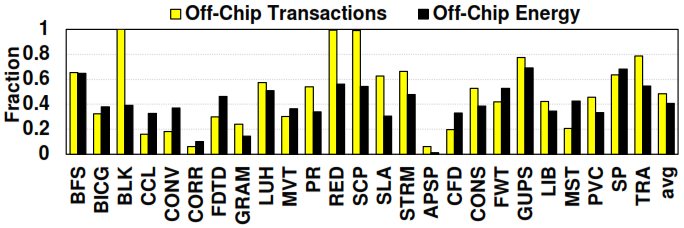
\includegraphics[scale=0.43]{figures/energy_consumption.png}
  \caption{Data movement and system energy consumption caused by off-chip memory accesses}
  \label{fig:power-consumption}
\end{figure}

Figure \ref{fig:power-consumption} illustrates the data movement and energy consumption overheads of transferring data between memory and compute units across 25 applications in a modern computer system, by showing: ($1$) the fraction of all data movement in the system stemming from off-chip transactions between memory and compute units, and ($2$) the fraction of total system energy consumption caused by this off-chip data movement. We notice that memory accesses result in $49\%$ of all data movement and are responsible for $41\%$ of the energy consumption of the system.

As such, developing a more advanced architecture has been urged for a quite long time to eradicate all issues caused by data movement in the traditional Von Neumann architecture. A promising approach is to move the processing closer to the memory to achieve faster access and higher bandwidth. Therefore, Processing in-memory and Near-Data Computing, which comply with such principle, come into sight as expected. We discuss this concept in the following sections.

\subsection{\bf Resurgence of \textit{Near-Data Computing}}
The concept of \textit{Processing in Memory} (PIM) or \textit{in-Memory Processing} is not novel, the original idea of implementing PIM dates back to early 1990's \cite{Kogge:1994:ENA:1260980.1261010, Gokhale:1995:PMT:618996.620191, Hall:1999:MIA:331532.331589, Patterson:1997:CIR:623274.624083, 808425, 748803}, and multiple PIM prototypes were proposed and demonstrated the potential for significantly improved performance and reduced power consumption in many application categories. Among them, EXECUBE \cite{Kogge:1994:ENA:1260980.1261010}, IRAM \cite{Patterson:1997:CIR:623274.624083}, DIVA \cite{Hall:1999:MIA:331532.331589}, FlexRAM \cite{808425} etc. are the representative early proposals. Efforts such as IRAM \cite{Patterson:1997:CIR:623274.624083} integrated embedded DRAM on logic chips. However, this approach was constrained by high-cost and low-density of the embedded DRAM, therefore it could not accommodate sufficient memory capacity and this drawback hindered its employment on high-performance systems.  Efforts such as DIVA \cite{Hall:1999:MIA:331532.331589} and FlexRAM \cite{808425} integrated logic on memory dies. However, due to the generation gap between DRAM processes and contemporary logic processes, the performance of logic implemented in DRAM processes was drastically reduced.

After a dormant decade for the PIM, recent advances in die-stacking technology extend memory systems from 2D planar structure to 3D stack structure \cite{Papanikolaou:2010:TDS:1965079, 6176900, 6131504}, which dramatically alleviate the cost limitation and practicality concerns of PIM. The success in commercialization of 3D stack memory system makes people thinking of the reincarnation of PIM \cite{Micron, AMD}. And this results in an upward trend in \textit{Near-Data Computing} (NDC) research field, and NDC has assumed a scope broader than that captured by the early PIM research of the 1990s.

%\subsection{Classification of Processing in Memory}

\section{Architecture of Near-Data Computing}
\textit{Near-Data Computing} (NDC), as its name suggested, applies the underlying principle \textit{processing in the proximity of memory} to minimize the data transfer cost, where monolithic compute units are physically placed closer to monolithic memories. 3D stacking technology is the most promising solution to bring computation as close as possible to data. Therefore, recently-proposed NDC hardware architectures use a similar base design, and a baseline node configuration suitable for \textit{Near-Data Computing} is shown in Figure \ref{fig:baseline} from a high-level view.

\begin{figure}[ht]
  \centering
  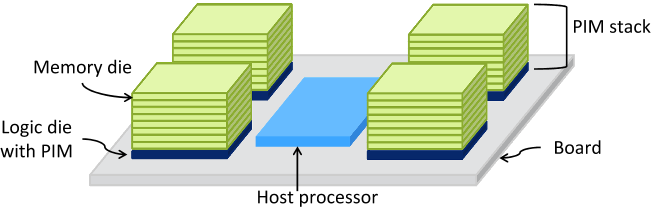
\includegraphics[scale=0.35]{architecture.png}
  \caption{An baseline configuration of compute node with PIM}
  \label{fig:baseline}
\end{figure}

Basically, an individual compute node of a \textit{Near-Data Computing} system consists of three entities: multiple memory stacks constitute the memory sub-system; a logic layer consisting of low-power \textit{compute units} beneath each memory stack acts as an accelerator; and a high-end host processor chip with high-performance cores takes charge of coordination among entities. The memory layers in a memory stack and the logic layer under this memory stack are integrated vertically by Through-Silicon-Via (TSV) technology. TSVs are used to ship data from the DRAM dies to the logic layer. Due to the extension to the third dimension, it allows the system to eliminate the energy overheads of moving data over long board traces, and also provides an order of magnitude higher bandwidth between the stacked memory banks and the compute units in the logic layer. The logic layer also implements high-speed signaling circuits so that it can interface with the host processor chip through fast and wide serial links. For power-efficient execution of complex analytics workloads like large-scale graph processing algorithms, it is best to use as large a number of low energy-per-instruction (EPI) cores as possible in logic layer. This will maximize the number of instructions that are executed per joule, and will also maximize the number of instructions executed per unit time, within a given power budget. We call these power-efficient cores in a logic layer the \textit{Near-Data Cores} or \textit{NDCores}. While the high-end host processor is packed together with those memory stacks on the same board. The high-end host processor is taking the charge of dispatching the tasks to NDCores and schedules the ordering of task dispatches.

Now let us look at more details of each subsystem in the following subsections.

\subsection{\bf Memory Stack}
Two most prominent and successfully commercialized 3D stacked memory technologies today are Micron's Hybrid Memory Cube (HMC) \cite{HMC-2.1} and JEDEC's High-Bandwidth Memory (HBM) \cite{HBM}. Although these two memory technologies have a few differences in physical structure and process. But from architectural and logical view they adopt the same memory organization, both HMC and HBM integrate a logic die with multiple DRAM chips in a single stack, which is divided into multiple independent channels (typically 8 to 16), as shown in Figure \ref{fig:3dstack}.

\begin{figure}[h]
	\centering
  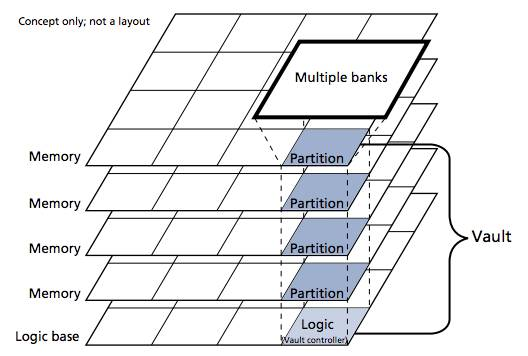
\includegraphics[scale=0.3]{hmc_concept.jpg}
  \caption{Architectural view of 3D stacked memory with logic layer}
  \label{fig:3dstack}
\end{figure}

Take HBM as example, it exposes each channel as a raw DDR-like interface; HMC implements DRAM controller in the logic layer as well as SerDes links for off-stack communication. The term \textit{vault} is used to describe the vertical channel in HMC, including the memory banks and its separate DRAM controller. 3D-stacked memory provides high bandwidth through low-power TSV-based channels, while latency is close to normal DDR3 and DDR4 chips due to their similar DRAM core structures \cite{6757501}.

\begin{table}[h]
\centering
\caption{Memory Technology Comparison \
        (based on data provided by Micron \cite{HMC-1.0})}
\label{tab:table1}
\begin{tabular}{|l|l|l|l|l}
\cline{1-4}
     & Pins & Bandwidth & Power  &  \\ \cline{1-4}
DDR3 & 143  & 12.8 GB/s & 6.2 W  &  \\ \cline{1-4}
DDR4 & 148  & 25.6 GB/s & 8.4 W  &  \\ \cline{1-4}
HMC  & 128  & 80.0 GB/s & 13.4 W &  \\ \cline{1-4}
\end{tabular}
\end{table}

\subsubsection{\bf Physical Characteristics of 3D-stacked Memory}
In Table \ref{tab:table1}, it illustrates a comparison between DDR3, DDR4, and HMC-style baseline designs from three aspects, in terms of power, bandwidth, and pin-count. 3D stacked memory, which has better bandwidth-per-pin and bandwidth-per-watt characteristics than either DDR3 or DDR4, is optimized for high-bandwidth operation and targets workloads that are bandwidth-limited. According to the HMC 1.0 specification \cite{HMC-1.0}, a single HMC provides up to 320 GB/s of \textit{external} memory bandwidth through eight high-speed serial links. On the other hand, a 64-bit vertical interface for each DRAM partition or \textit{vault}, 32 vaults per cube, and 2 Gb/s of TSV signaling rate \cite{Pugsley2014NDCAT} together achieve an \textit{internal} memory bandwidth of 512 GB/s per cube. Moreover, this gap between external and internal memory bandwidth becomes much wider as the memory capacity increases with the used of more HMCs. The key objective of adopting near-memory processing is not solely to provide high memory bandwidth, but especially to achieve \textit{memory-capacity-proportional} bandwidth. Considering a system composed of 16 8GB HMCs as an example, conventional processors are still limited to 320 GB/s of memory bandwidth assuming that the CPU chip has the same number of off-chip links as that of an HMC. In contrast, a NDC system exposes 8 TB/s (=16 $\times$ 512 GB/s) of aggregate internal bandwidth to the in-memory computation units. This memory-capacity-proportional bandwidth facilitates scaling the system performance with increasing amount of data in a cost-effective way, which is a key concern in irregular data access patterns, such as graph processing \cite{Ahn:2015:SPA:2749469.2750386}.\\

% \subsubsection{\bf Memory Addressing in NDC}
% Most of \textit{Near-Data Computing} systems don't provide \textit{virtual memory} mechanism although the main memory of host processors may support it. This is because the \textit{NDCore} acts like an accelerator that is memory-mapped to part of a non-cacheable memory region of the host processors. Without supporting virtual memory, it eliminates the need for managing \textit{cache coherence} between caches of the host processor and the 3D-stacked memories. From the application perspective, such as big data, graph processing, deep learning, etc. they usually do not require functionality provided by virtual memory. Furthermore, without equipping virtual memory avoids the need for address translation inside memory which causes non-trivial performance overhead.

\begin{figure}
    \center
    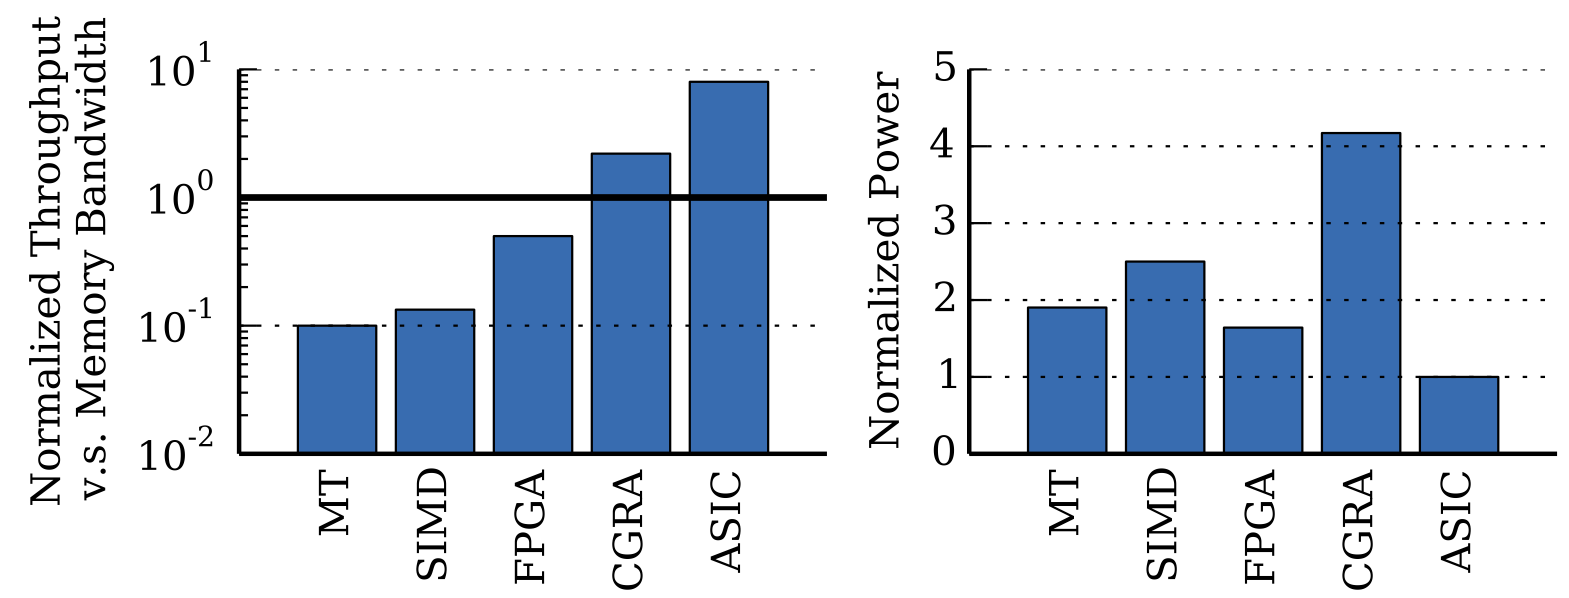
\includegraphics[scale=0.20]{figures/comparison_ndcores.png}
    \caption{Computational throughput and power consumption for different logic types implementing the graph processing kernel: multi-threaded (MT) cores, SIMD cores, FPGAs, CGRAs, and custom units (ASICs).}
    \label{fig:NDC-comparison}
\end{figure}

\subsection{\bf Logic Layer and Compute Units}
The logic layer at the bottom of 3D-stacked memory contains the \textit{Near-Data Cores} (or \textit{NDCores}) and is the key component to fulfill the \textit{Near-Data Computing}. It is also where an outstanding design distinguishes from others. These NDCores should (1) be \textit{area-efficient} in order to provide sufficient computational throughput to match the high bandwidth available through 3D stacking; (2) be \textit{power-efficient} in order to reduce total energy consumption, and to avoid causing thermal issues in the DRAM stacks; (3) provide \textit{high flexibility} to allow for reuse across multiple applications and applications domains. Recently proposed designs implement the compute units inside a \textit{NDCore} with simple cores, SIMD units, GPUs, FPGA blocks, CGRA arrays, or custom accelerators (ASICs).

Figure \ref{fig:NDC-comparison} compares different logic options available to NDC systems on which a typical kernel of graph processing is executed \cite{7446059}. To be fair in this experiment, all these options utilize the same memory configuration. Each memory stack possesses 8 vaults (or channels) and supplies up to 128 GBps peak bandwidth in total, but, once memory controllers and interfaces are accounted for, only about 50 $mm^2$ of the logic layer can be used for compute units \cite{6242474}. Whenever the area and power budgets allow it ought to put as many logic units as possible in the stack. The computational throughput in Figure \ref{fig:NDC-comparison} is normalized to the maximum memory bandwidth, indicated by the solid line. Matching this line implies a balanced system with sufficient compute capability to take full advantage of the high bandwidth through TSVs. Once the memory bandwidth is saturated there is no point in scaling the computational throughput any further.

\subsubsection{\bf General-purpose Processor as NDCore}
This category of \textit{NDCores} design takes the same philosophy as \textit{many-core processor} design. The logic layer under the 3D-stacked memory contains one simple processor core for each vault; as we previously mentioned, one stack has 32 vaults, therefore, each stack holds 32 cores \cite{Pugsley2014NDCAT, Ahn:2015:SPA:2749469.2750386}, a typical design is shown in Figure \ref{fig:tesseract}.
\begin{figure}[h]
  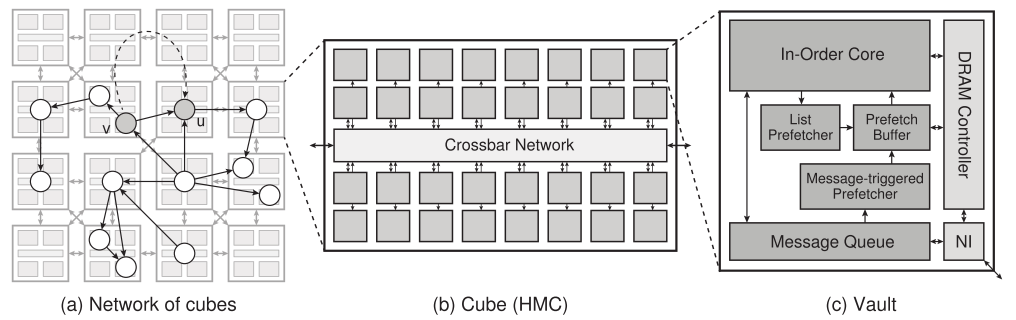
\includegraphics[scale=0.33]{figures/tesseract_2.png}
  \caption{A typical NDC system with general-purpose processor cores as \textit{NDCores} \cite{Ahn:2015:SPA:2749469.2750386}.}
  \label{fig:tesseract}
\end{figure}
\textbf{The architecture of NDCore.} Most designs which fall into this category use simple in-order cores similar to ARM Cortex-A series as \textit{NDCores} \cite{ARM-Cortex-A5, ARM-Cortex-A7}, such as the one shown in Figure \ref{fig:tesseract} (c). Wide-issue or Out-of-Order cores are not necessary due to the lack of temporal locality and abundant instruction-level parallelism in code, nor are they practical given the stringent power and area constraints. For some workloads -- particularly for irregular and unbalanced workloads, such as graph processing -- some NDCores may suffer from underutilization as they are often stalled waiting for data processed by other NDCores. Therefore, fine-grained \textit{multi-threading} (cycle-by-cycle) should be used as a cost-effective way to improve the utilization of simple cores given a considerable amount of memory bandwidth available within each stack \cite{Alverson:1990:TCS:77726.255132, Gao2015}.

\textbf{The communication among NDCores.} Another matter for \textit{NDCores} of this category is the handling of communication among cores internally in a stack and externally between stacks, respectively. Many real-world applications, such as graph processing and deep learning, require complex communication between hundreds to thousands of threads \cite{Gonzalez:2012:PDG:2387880.2387883, Chilimbi:2014:PAB:2685048.2685094}. Relying on the host processor to manage all the communication will not only turn it into the performance bottleneck but will also waste energy moving data between the host processor and memory stacks.\\
To solve this issue, some elegant solutions are proposed. Tesseract \cite{Ahn:2015:SPA:2749469.2750386} employs a low-cost message passing mechanism plus prefetching for communication between \textit{NDCores}. Tesseract chooses message passing to (1) avoid cache coherence issues, (2) eliminate the need for locks to guarantee atomic updates of shared data, and (3) overlap the message passing with computation to hide the latency of remote access. While, another design \cite{Gao2015} proposes a per-core \textit{remote load buffer} (RLB) mechanism, that allows sequential prefetching and buffering of a few cache lines of \textit{read-only} data. This is manageable because flushes are only necessary at synchronization points such as barriers, as a result no writeback is needed.

\subsubsection{\bf Accelerator as NDCore}
\textit{Near-Data} cores composed by SIMDs (mostly GPUs) or ASICs are considered as accelerators. Both SIMD or ASIC architecture is suitable for specific fields of applications opposite to general purpose ones, thus it is appropriate to put them into accelerator category.

\begin{figure}[h]
  \center
  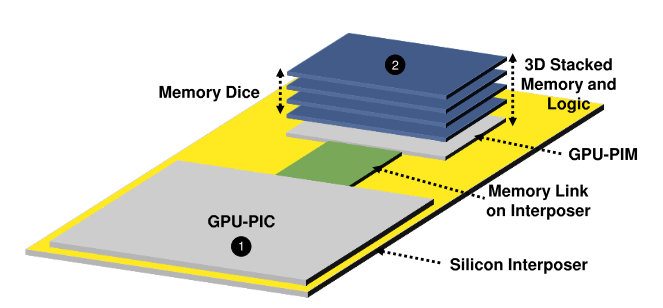
\includegraphics[scale=0.40]{figures/ndc_gpu.png}
  \caption{NDC-assisted GPU architecture \cite{7756764}}
  \label{fig:NDC-gpu}
\end{figure}

\textbf{GPU core as NDCore}. A GPU-based NDC system consists of at least one 3D-stacked memory chip and a powerful GPU chip placed adjacent to memory stack, the 3D-stacked memory integrates a base logic layer, housing a chip with GPU cores. Both chips are interconnected through a high-speed serial memory link on an interposer, as demonstrated in Figure \ref{fig:NDC-gpu}. This architecture contains two types of compute engines: $\left(1\right)$ large and powerful primary GPU cores, which is similar to modern GPU cores, and $\left(2\right)$ smaller and less powerful GPU cores, which are placed in the logic layer under 3D-stacked memory and assist in performing the computation. The GPU integrated into memory stack is more power-efficient than the main GPU and this organization has considerably lower thermal constraints and is more scalable in terms of memory capacity. In order to fully and automatically exploit the performance and energy-efficiency of the system, mechanisms of how to automatically identify the code segments to be offloaded to the GPU cores in memory stack are needed. Also to maximize the concurrency, a smart strategy has to be adopted for scheduling multiple kernels on the main GPU and the cores in memory. For example, computations that are memory-intensive and can tolerate the lower parallelism presenting in the logic layer of GPUs are likely better executed on GPU cores in memory stack instead of on main GPU.

\textbf{ASIC as NDCore}. In Figure \ref{fig:NDC-comparison}, custom accelerators (ASICs) shows an extreme, they can easily saturate the memory channels but lack programmability. The extra compute capability provides marginal benefits \cite{7446059, Loh2013APT}. ASICs are usually made for digital signal processor (DSP), and they provide very small silicon footprint and much lower power consumption compared to other types of NDCores.

Due to limited functionalities of ASICs, there is only a small number of designs considering to adopt ASICs in NDC system, however their stunning performance and low power potential still attract research on some specific applications. A typical example is the customized compute engine designed for MapReduce framework. Both \textit{Mapper} and \textit{Reducer} phases need large quantities of sorting operations, so a customized sorting engine will offer great help. \cite{Pugsley2015FixedfunctionHS} presents the hardware accelerator for merge sort and bitonic sort. The merge sorter follows the \textit{divide and conquer} paradigm and is internally organized like a heap, and each cycle the smallest of two input key-value pairs will be chosen to advance to the next level; the input stream buffers must keep track of the sorted input lists. Merge sorters are mainly used for small size input, each merge sorter works on an input with 2 to 8 elements. On the other hand, A bitonic sorter can sort 1024 inputs, and it is either used as a finishing step to finalize the sorting that has been partially accomplished by a hardware range partitioning unit, or used as a pre-processing step to prepare an input to be operated on by a group of eight-input hardware merge sorters.

\subsubsection{\bf Reconfigurable Compute Unit as NDCore}
The third category of logic units available to be used in a logic layer are reconfigurable units, they provide a good trade-off between performance and flexibility. There are two common reconfigurable logic types, FPGA and CGRA.

\textbf{Architectural View of Reconfigurable Compute Unit.} FPGA achieves low power consumption through customization but suffers from low clock speed and high area overheads due to the bit-level configurable blocks and routing fabric, which are too fine grained for arithmetic operations, The DSP blocks in modern FPGAs help unless their number and width match emerging big data applications. This is one drawback shown in the left diagram of Figure \ref{fig:NDC-comparison}, it indicates that FPGA may fail to saturate memory bandwidth with high performance under the area constraints.

\begin{figure}[h]
  \centering
  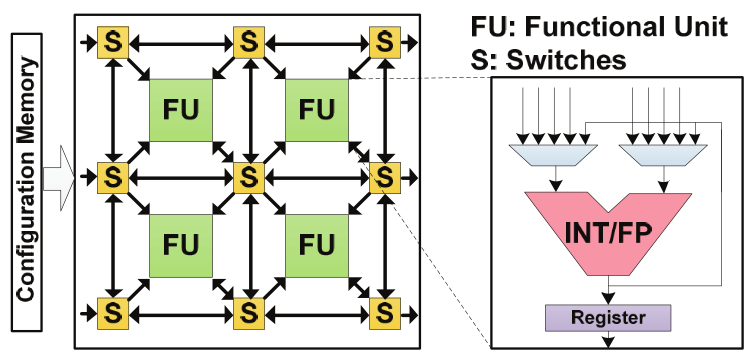
\includegraphics[scale=0.35]{figures/nda.png}
  \caption{A CGRA with a grid of 2$\times$2 functional units \cite{7056040}.}
  \label{fig:nda}
\end{figure}

Another type of reconfigurable compute units, called \textit{Coarse-Grain Reconfigurable Accelerators} (or CGRAs), can be deployed to the logic layer of a memory stack. A CGRA is typically comprised of a large number of coarse-grained functional units (FUs) in a grid which perform various arithmetic and logic operations, which are connected by a configurable interconnect fabric (Figure \ref{fig:nda}); CGRAs also significantly reduce the power and area overheads for computation. However, due to the limitation of the simple interconnect, traditional CGRAs only target applications with regular computation patterns, such as matrix multiplication or image processing. Recent NDC systems \cite{7056040, 7446059} used some new types of CGRA with either circuit-switch routing network \cite{7056040} or CLB \cite{7446059} as a powerful interconnect to support more complicated data and control flows. The CLBs in  \cite{7446059} (Figure \ref{fig:hrl}, which the author calls it \textit{Heterogeneous Reconfigurable Logic}), are similar to those in FPGAs, they utilize lookup tables (LUTs) for arbitrary, bit-level logic. With the help of these CLBs, the NDCores can implement control units which are less regular, e.g. load and store unit with indirect addressing mode used in data access pattern of sparse structure.

\begin{figure}[h]
  \centering
  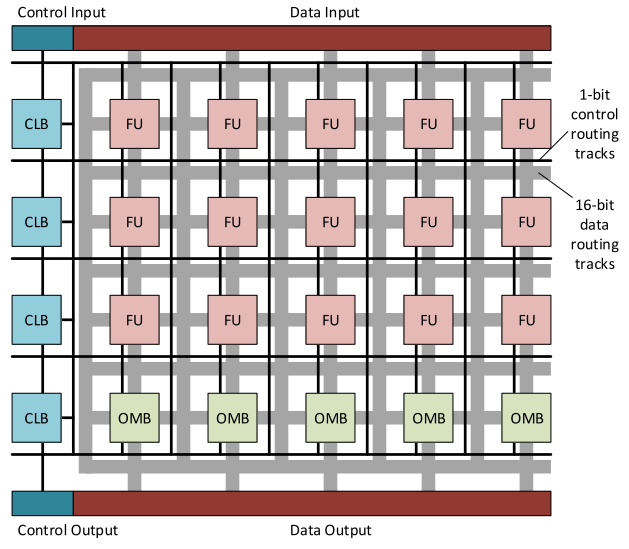
\includegraphics[scale=0.35]{figures/hrl.png}
  \caption{The organization of the Heterogeneous Reconfigurable Logic (HRL) array \cite{7446059}}
  \label{fig:hrl}
\end{figure}

\textbf{Computational Model of Reconfigurable Compute Unit.} Data-intensive and compute-intensive application kernel can be decomposed into \textit{dataflow graphs}. A \textit{dataflow graph}, containing nodes (operations) and edges (data transfer or communication), is mapped to the FPGA's DSP or CGRA's FUs and interconnect either manually or using automated techniques. The host processor triggers FPGA or CGRA reconfiguration at runtime to implement different kernels at different times, replacing the content of configuration memory with the new dataflow graph's configuration data. Exploiting spatial data parallelism in application kernels and efficiently processing kernel's dataflow graphs; reconfigurable compute unit, e.g. CGRAs, considerably improve performance and energy consumption compared to conventional processors, as shown in Figure \ref{fig:NDC-comparison}. In particular, CGRAs can partially eliminate the large energy overheads of fetching and scheduling instructions in conventional out-of-order processors. While, FPGA alike logic, e.g. CLBs in FPGA, provides more flexible programmability in interconnect.

\subsection{Host}
Most NDC system use a high-end processor with out-of-order (OoO) cores as host, while GPU NDC system uses advanced and powerful GPU as host. As stated in previous section, most of NDCores don't support virtual memory, nevertheless, host processors can still use virtual addressing in their main memory since they use separate DRAM devices. Since host processors have access to the entire memory space of system, including 3D-stacked memory, it is up to the host processors to distribute workloads across HMC vaults.

\section{Performance and Energy Analysis}
\begin{figure*}[h]
    \centering
    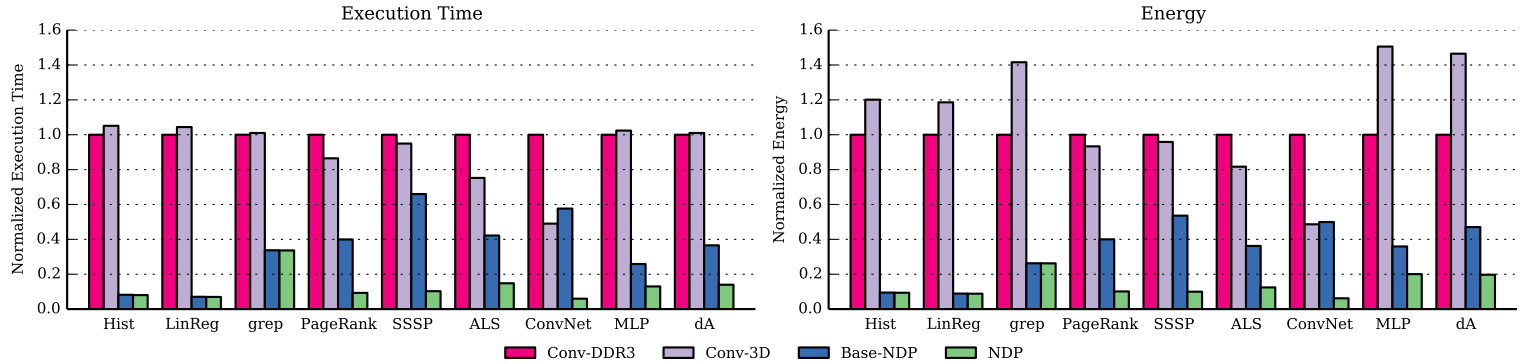
\includegraphics[width=\textwidth, scale=0.5]{figures/comparison_performance_energy.png}
    \caption{Performance and energy comparison between Conv-DDR3, Conv-3D, Base-DNC and advanced DNC systems \cite{Gao2015}.}
    \label{fig:comp-power-energy}
\end{figure*}
The work in \cite{Gao2015} shows the experiment on power and performance comparison. The authors used a conventional DDR3 system as a baseline (Conv-DDR3), they made comparison among the system of 3D stacking without logic layer (Conv-3D), the base NDC system, and an advanced NDC system (2 threads per vault, 16 vaults per stack, 8 stacks, 1024 threads in total). Figure \ref{fig:comp-power-energy} illustrates the performance and energy comparison between the above four systems. The Conv-3D system supplies significantly higher bandwidth than the DDR3 baseline due to the use of high-bandwidth 3D memory stacks. However, the two NDC systems deliver significant improvement over both the Conv-DDR3 and the Conv-3D systems in terms of performance and energy. The base-NDC system achieves around 3.5$\times$ faster 3.4$\times$ more energy efficient over DDR3 baseline. The advanced NDC system attains another 2.5$\times$ improvement over the base-NDC and accomplishes 3-16$\times$ better performance and 4-16$\times$ less energy over the base-DDR3 system.

Both NDC systems consume significantly low energy due to that 3D-stack memory removes the distance of data transfer across long traces on board. Another factor affects energy rising from DDR memory's dynamic recharging; highly-threaded multi-core/many-core architecture can greatly reduced the total cycles of execution, hence, NDC systems eliminate much more stalled cycles where dynamic energy dissipation happen. The improvement in speed for both NDC systems is obvious, \textit{higher bandwidth} and \textit{shorter distance} for data transfer play crucial roles.

\section{Algorithmic Level Optimization}
Balancing workloads in vaults and reducing nontrivial data transfers among vaults are two critical issues which seriously affect the performance and power consumption of NDC systems. Workload balancing concerns how computation is distributed to each vault and how data is partitioned and processed then stored in each vault. Whenever it is necessary, one vault may need to access the data stored in another vault to continue its own computation; each request and response pair for data transfer involves non-trivial communication through memory banks and a serial link between memory stacks and costs power consumption while transmission of data and signaling. So workload balancing and non-trivial communication reduction are very important for NDC system design as well as in software level.
\subsection{Data Partition and Workload Balancing}
A Better data partitioning for balancing workload on each NDCore can effectively improve the overall performance of system by $\left(1\right)$ getting a higher concurrency, $\left(2\right)$ reducing the total amount time when some NDCores are idle while others are engaged in performing some tasks, and $\left(3\right)$ minimizing the number of data transfers between different vaults.

The workload balancing can be broadly classified into two categories: \textbf{\textit{static}} and \textbf{\textit{dynamic}}. Static workload balancing strategy is simple to realize with the help of the compiler and the OS, for many practical cases, relatively inexpensive heuristics provide fairly acceptable approximate solutions to the optimal static workload balancing problem. While dynamic balancing strategy can be more flexible and versatile, especially when static strategy may result in a highly imbalanced distribution of data and workload partition. However, it is more complicated to realize a dynamic strategy and also requires some hardware modifications to support those mechanisms used in the dynamic strategy.

\subsection{\bf Case studies}
In the following subsection, we give some case studies to show how workload balancing and algorithmic level optimization affect the performance and power consumption of NDC system.

\subsubsection{\bf Case 1: Static workload balancing in graph processing}
Sequential memory access pattern provides the most energy efficient way to exploit spatial locality, further maximizes the cache utilization, avoids remote data transfer between NDCores, and also reduces the energy overhead of fetching cache line; these merits are all expected by graph processing. Figure \ref{fig:graph-vertex-edge} compares the performance, energy, cache line utilization, and DRAM row utilization of two implementations of a graph framework (The kernel of the framework is an implementation of \textit{Single Source Shortest Path} (or \textit{SSSP}) algorithm). The edge-centric implementation provides a $2.9\times$ improvement in both performance and energy over the vertex-centric. The key advantage is that the edge-centric scheme enhances spatial locality (streaming, sequential accesses). The cache line utilization histogram indicates that the higher spatial locality is converted into a higher fraction of the data used within each cache line read from memory, and a lower total number of cache lines that need to be fetched \cite{Gao2015}.

\begin{figure}[h]
  \centering
  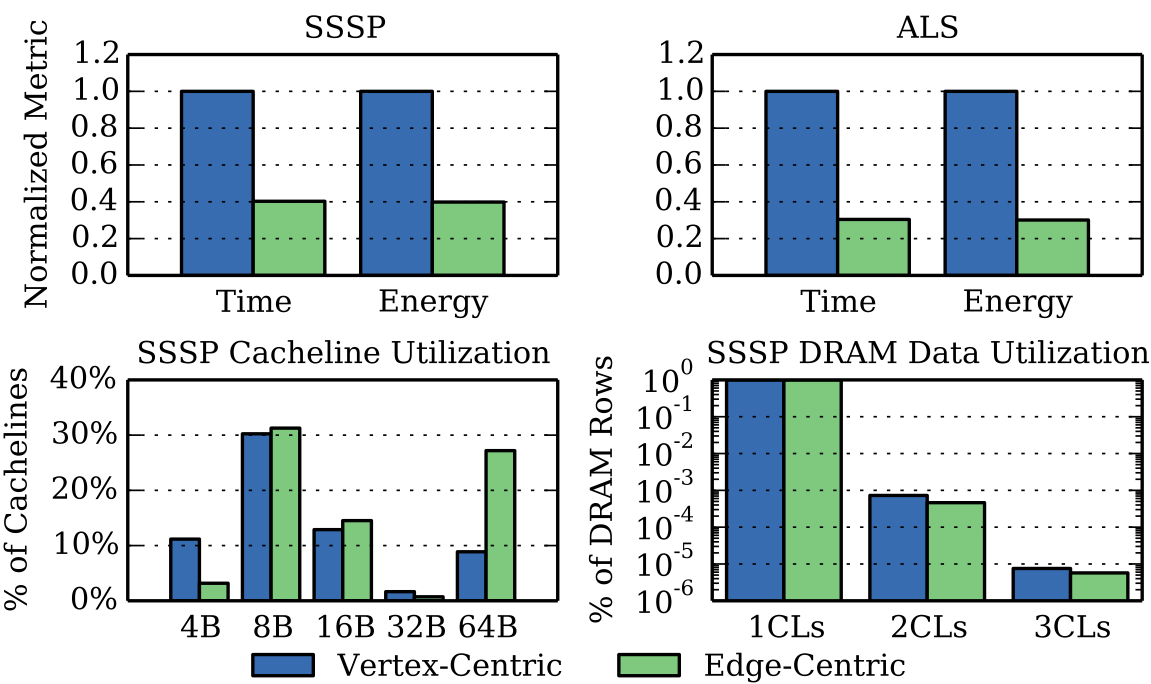
\includegraphics[scale=0.29]{figures/ndc_graph_vertex_vs_edge.png}
  \caption{Vertex-centric and edge-centric graph frameworks. \cite{Gao2015}}
  \label{fig:graph-vertex-edge}
\end{figure}

From the algorithmic perspective, in each iteration SSSP searches for the edge to a vertex that appears closest to a source. Vertex-centric graph partitioning divides the set of vertices (adjacent lists) into several partitions then loads them in the vaults of the memory stack. SSSP needs to frequently access the weight information of edges. When two vertices of an edge were dispatched in different vaults (as shown in Figure \ref{fig:tesseract}), the remote request for weight information sent to these two vaults is inevitable. The action of sending request costs delay while waiting for the reply and eventually the degradation of performance. It will be even worse when too many remote requests are issued then the resulting communication congestion deteriorates performance and power consumption. On the other hand, edge-centric implementation can avoid unnecessary remote requests for edge information since the necessary information stored in the same vault, therefore cross-vault communications issued by an edge-centric implementation are less than the counterpart. Of course, edge-centric implementation has its own drawback, that is, the data structure used by edge-centric implementation requires redundant storage. Therefore, this overhead occupies more storage space in each vault.

\begin{figure}[h]
  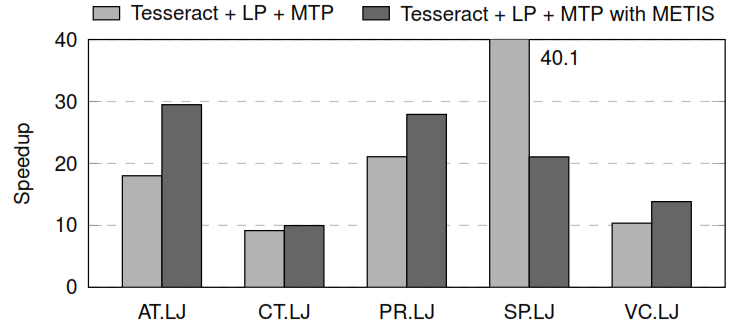
\includegraphics[scale=0.4]{figures/graph_partition_optimization.png}
  \caption{Performance improvement after graph partitioning. \cite{7284059}}
  \label{fig:graph-partition}
\end{figure}

Elaborate graph partitioning schemes should be employed for balancing the workload in each vault. A better data partitioning can minimize communication between different vaults and between different memory stacks. Figure \ref{fig:graph-partition} shows the performance improvement of Tesseract \cite{7284059} where the input graphs are evenly distributed across vaults based on an optimized graph partitioning algorithm. For the purpose of shortening the critical path (the more workload are balanced, the shorter the critical path), the author employs METIS \cite{Karypis:1998:FHQ:305219.305248} to perform 512-way multi-constraint partitioning to balance the number of vertices, outgoing edges, and incoming edges of each partition. Therefore, employing better graph distribution can further improve the performance of NDC system. This is because graph partitioning minimizes the number of edges crossing between different partitions ($53\%$ fewer edges cuts compared to random partitioning in LJ as shown in Figure \ref{fig:graph-partition}), and thus, reduces off-chip network traffics.

\subsubsection{\bf case 2: Dynamic Strategy of Workload Balancing}
Dynamic workload balancing techniques are usually used for the applications with the unpredictable workload at runtime. And in some cases, the workload can also be generated dynamically, e.g. reinforcement learning problems. In the work of \cite{7284059}, the author proposed a dynamic strategy which offloads workload to NDC-assisted GPU platform. Their strategy first divides the workload according to the \textit{computational kernels}, these kernels will be executed concurrently. Furthermore, each kernel takes different execution time on NDCore from on main GPU (recall in section II.B.2, the GPU-based NDC system consists of a powerful main GPU (or GPU-PIC, PIC stands for Processing in core), and a single memory stack or several memory stacks integrated with low-power simple GPU cores (NDCores or GPU-PIM, PIM stands for processing in memory)). Therefore, to make the workload executed fast and efficiently on this GPU-based NDC system, we need to conceive an algorithm to offload each kernel of the workload to an appropriate compute node, either on main GPU or on the NDCores.

Figure \ref{fig:gpu-offload} illustrates the advantage of kernel offloading over application offloading for FDTD (Finite-Difference Time-Domain) application. Scenario-$I$ and Scenario $II$ are the two possible application offloading strategies executing the entire FDTD application on GPU-PIM or GPU-PIC, respectively. On the other hand, in the kernel offloading strategy (Scenario-$III$), each \textit{kernel} of FDTD is offloaded to the computation engine where its execution time is lower (i.e., each kernel is offloaded to a unit it has \textit{affinity} towards). Therefore, Kernel-K1 is offloaded to GPU-PIM and the other two kernels are offloaded to GPU-PIC. Kernel offloading saves many execution cycles (\Circled{A}) even beating the best application offloading strategy. However, the key challenge of kernel offloading is in identifying the \textit{affinity} of each kernel.
\begin{figure}[ht]
  \centering
  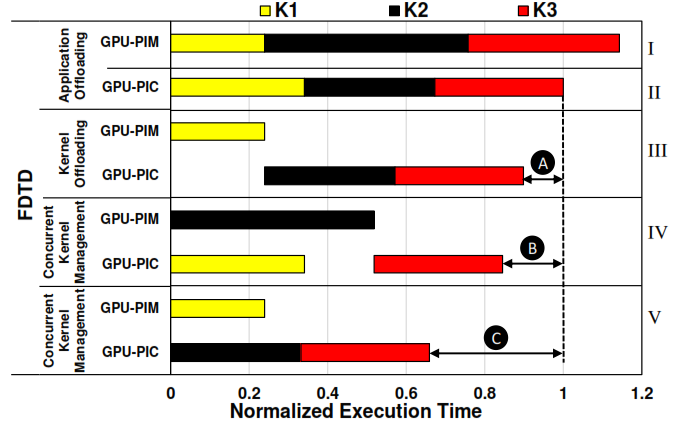
\includegraphics[scale=0.4]{figures/gpu_offload.png}
  \caption{Performance advantages of kernel offloading ($III$) and concurrent kernel management ($IV$ and $V$) mechanisms using the FDTD application as an example}.
  \label{fig:gpu-offload}
\end{figure}
Another benefit of the offloading workload in kernel level is that we can manage the kernel scheduling at fine-grained granularity. Whenever the kernels are independent, they can be executed concurrently by utilizing as many compute units as possible. Figure \ref{fig:gpu-offload} demonstrates an example of this in Scenario $IV$ and Scenario $V$. In FDTD, Kernel-K3 depends on both Kernel-K1 and Kernel-K2, so it can begin only when both Kernel-K1 and Kernel-K2 have done their executions. However, Kernel-K1 and Kernel-K2 can execute in parallel. Due to the concurrent execution of kernels, overall application execution time is decreased (\Circled{B}), compared to the best application-offloading scenario, in scenario-$IV$. Scenario-$V$ in Figure \ref{fig:gpu-offload} illustrates that kernel affinity, i.e., scheduling each kernel on the execution engine that is best for the kernel's performance matters: Kernels K1 and K2 have affinity for GPU-PIM and GPU-PIC, respectively. Further, executing them concurrently on these engines leads to even higher overall application execution time savings (\Circled{C}) than in Scenario-$IV$ where the same kernels are scheduled onto the opposite engines.

\section{CONCLUSIONS}
In this paper we revisit the \textit{Near-Data Computing} (NDC) system from the architectural and technological perspectives,  we also present case studies demonstrating performance optimization. As 3D integration technology becomes more and more mature and reliable, it is no longer the technical adoption barrier for implementing computer architecture with near memory computation ability. NDC offers a promising approach to overcome the challenges posed by emerging data-intensive applications. Moreover, a viable NDC system should be constructed by collaborative efforts between technologies, IC designers and system engineers, as what we have shown in case study sections. The simulation results show that NDC significantly improves the performance of a wide range of evaluated applications (3.2-60.6$\times$) and reduces their total energy consumption (63-96$\%$).

%\addtolength{\textheight}{-12cm}   % This command serves to balance the column lengths
                                  % on the last page of the document manually. It shortens
                                  % the textheight of the last page by a suitable amount.
                                  % This command does not take effect until the next page
                                  % so it should come on the page before the last. Make
                                  % sure that you do not shorten the textheight too much.

%%%%%%%%%%%%%%%%%%%%%%%%%%%%%%%%%%%%%%%%%%%%%%%%%%%%%%%%%%%%%%%%%%%%%%%%%%%%%%%%



%%%%%%%%%%%%%%%%%%%%%%%%%%%%%%%%%%%%%%%%%%%%%%%%%%%%%%%%%%%%%%%%%%%%%%%%%%%%%%%%



%%%%%%%%%%%%%%%%%%%%%%%%%%%%%%%%%%%%%%%%%%%%%%%%%%%%%%%%%%%%%%%%%%%%%%%%%%%%%%%%
%% \section*{APPENDIX}

% Appendixes should appear before the acknowledgment.

%%%%%%%%%%%%%%%%%%%%%%%%%%%%%%%%%%%%%%%%%%%%%%%%%%%%%%%%%%%%%%%%%%%%%%%%%%%%%%%%

% References are important to the reader; therefore, each citation must be complete and correct. If at all possible, references should be commonly available publications.



% \begin{thebibliography}{99}
% \bibitem{c1} Mingyu Gao, Grant Ayers, and Christos Kozyrakis. 2015. Practical Near-Data Processing for In-Memory Analytics Frameworks. In Proceedings of the 2015 International Conference on Parallel Architecture and Compilation (PACT'15).


% \end{thebibliography}
\bibliographystyle{ieeetr}
\bibliography{ref}

\end{document}
